\chapter{Dataset Understanding and EDA}\label{chap:eda}

% Helper: wrapped columns for neat 3-col tables
\newcolumntype{P}[1]{>{\raggedright\arraybackslash}p{#1}}

\section{Overview}
This chapter covers the data assets and clinical labeling used to build the analysis-ready SA--AKI cohort. It establishes the temporal conventions and data harmonization steps that precede the main analysis. Crucially, it then details the comprehensive Exploratory Data Analysis (EDA) conducted on the training set. This EDA serves as a form of unsupervised phenotyping, identifying the key clinical characteristics and risk factors that differentiate patient outcomes and providing the empirical foundation for the subsequent predictive modeling.

\section{Source Tables and Warehouse Context}
Figure~\ref{fig:data-universe} positions the raw inputs within MIMIC--IV (core, hosp, ICU) that were ingested and optimized in the warehouse. These tables provide the vitals, labs, medications, microbiology, and encounter scaffolding used for labeling and features.

\begin{figure}[htbp]
    \centering
    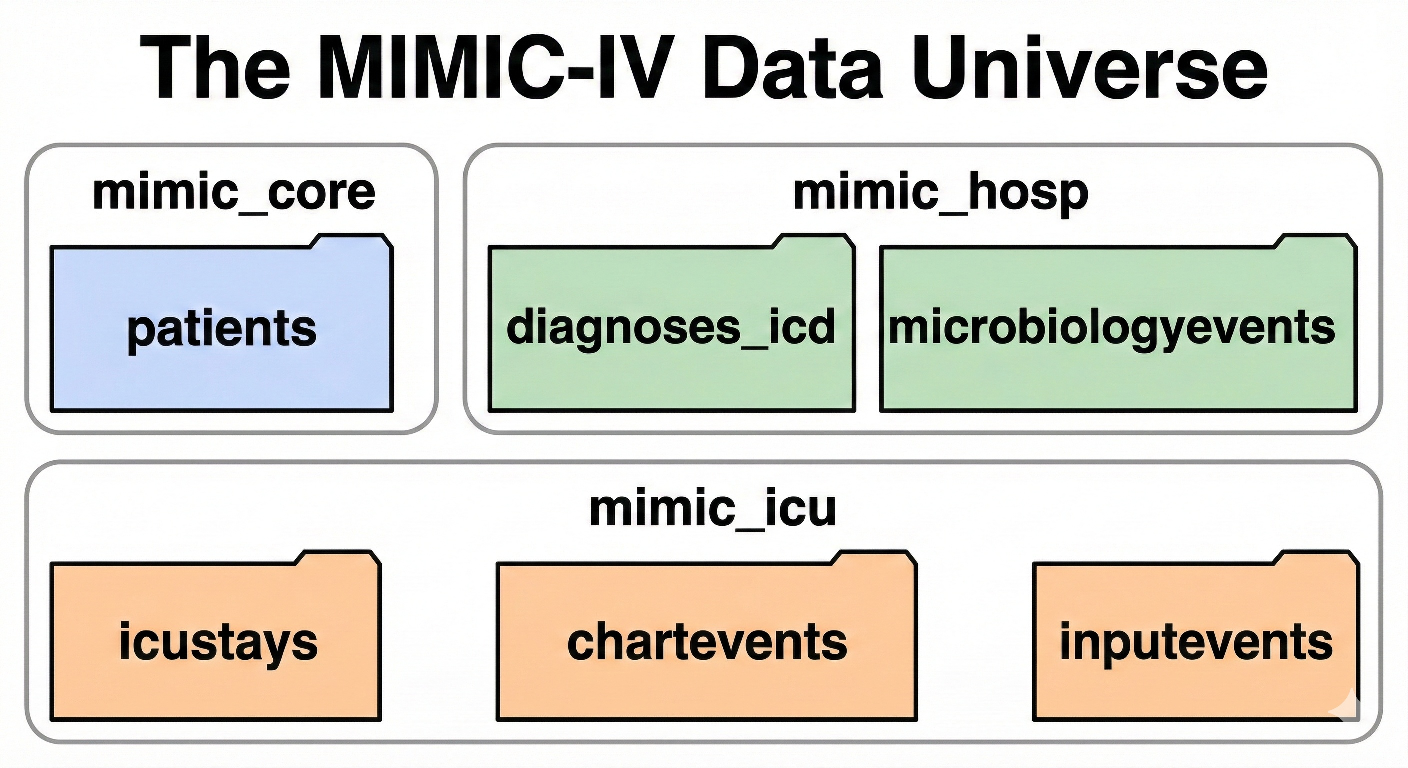
\includegraphics[width=\linewidth,height=0.85\textheight,keepaspectratio]{dataset_images/1_data_universe.pdf}
    \caption{MIMIC--IV data universe leveraged in this study.}
    \label{fig:data-universe}
\end{figure}

\section{Ontology-Driven Concept Identification}
To avoid brittle, hard-coded drug lists, we map clinical concepts across terminologies and derive ingredient-level value sets programmatically. The crosswalk in Figure~\ref{fig:ontology-crosswalk} shows the pathway from SNOMED~CT through UMLS CUIs into RxNorm ingredients, with ATC used as an orthogonal cross-reference and coverage check. This pipeline underlies the study’s systemic \emph{antibiotic} and \emph{vasopressor} flags used in labeling and feature construction.

\begin{figure}[htbp]
    \centering
    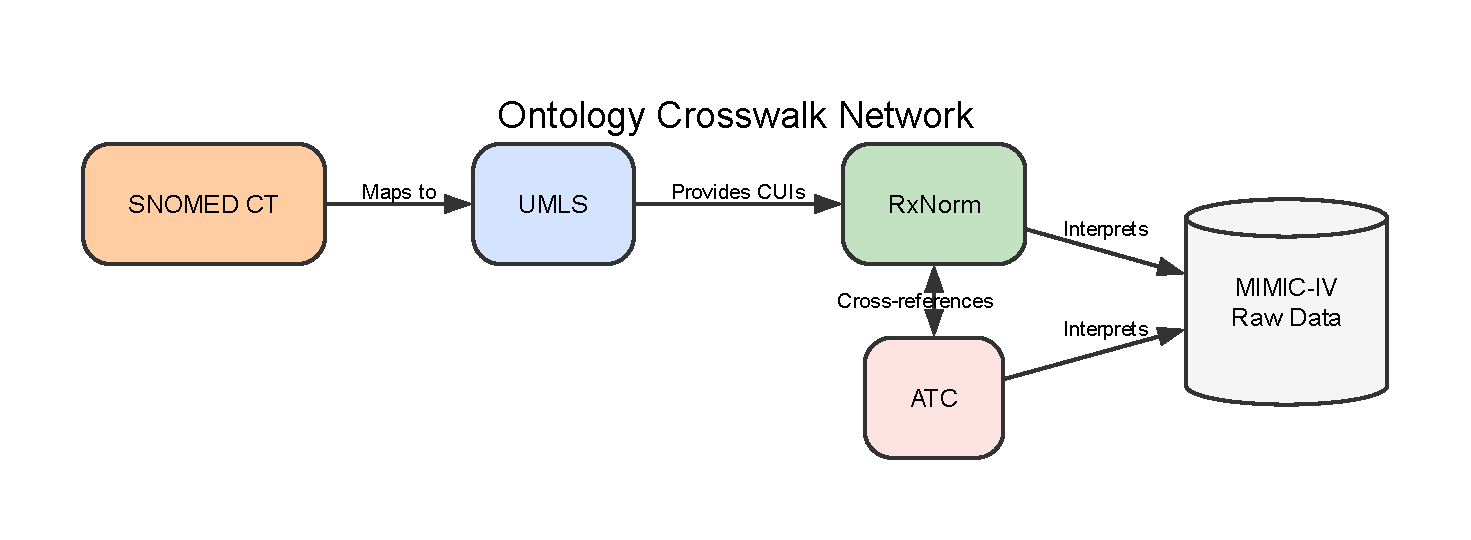
\includegraphics[width=\linewidth]{dataset_images/7_ontology_crosswalk}
    \caption{Ontology crosswalk linking SNOMED~CT $\rightarrow$ UMLS CUIs $\rightarrow$ RxNorm ingredients, with ATC cross-reference.}
    \label{fig:ontology-crosswalk}
\end{figure}

\section{Cohort Construction (Counts and Exclusions)}
We follow a CONSORT-style reduction from all ICU stays to the final analysis cohort. Figure~\ref{fig:consort} consolidates inclusion criteria (adult, first ICU stay, LOS~$\ge$~24\,h), Sepsis--3 screening, SA--AKI temporal linkage, and final exclusions (ESRD, early RRT). These counts are the reference for all summary denominators used in EDA.

\begin{figure}[htbp]
    \centering
    
\includegraphics[width=\linewidth,height=0.85\textheight,keepaspectratio]{dataset_images/8_consort_flow}
    \caption{CONSORT-style flow of cohort construction with key exclusions.}
    \label{fig:consort}
\end{figure}

\section{Clinical Labeling Rules and Time Anchors}
\subsection{Sepsis--3 and AKI Logic (Compact View)}
Sepsis--3 requires \emph{suspected infection} \emph{and} an acute increase in organ dysfunction ($\Delta$SOFA~$\ge$~2). AKI follows KDIGO using three criteria: serum creatinine (absolute/relative) and urine output (UO). We display the Sepsis--3 gate and the UO sessionization used for the KDIGO UO criterion as a two-panel composite in Figure~\ref{fig:logic-composite}.

\begin{figure}[htbp]
    \centering
    \begin{subfigure}{0.49\linewidth}
        \centering
        
\includegraphics[width=\linewidth,height=0.4\textheight,keepaspectratio]{dataset_images/10_sepsis3_and_logic}
        \caption{Sepsis--3 core logic gate.}
    \end{subfigure}\hfill
    \begin{subfigure}{0.49\linewidth}
        \centering
        
\includegraphics[width=\linewidth,height=0.4\textheight,keepaspectratio]{dataset_images/9_urine_output_logic}
        \caption{UO sessionization for KDIGO (continuous windows $<$0.5\,mL/kg/h for $\ge$6\,h).}
    \end{subfigure}
    \caption{Clinical rule components used for cohort labeling.}
    \label{fig:logic-composite}
\end{figure}

\subsection{Timeline Conventions and Windows}
All predictors used in modeling are restricted to the first 24\,h after ICU admission (T0--T24). Suspected infection is defined by a temporal link between cultures and systemic antibiotics, and SA--AKI requires AKI onset within $\pm$48\,h of Sepsis onset. Figure~\ref{fig:timeline} illustrates these anchors and windows.

\begin{figure}[htbp]
    \centering
    
\includegraphics[width=\linewidth,height=0.85\textheight,keepaspectratio]{dataset_images/6_final_timeline}
    \caption{Illustrative patient journey with T0--T24 feature window, infection window, Sepsis onset, and AKI onset; the SA--AKI link is $\pm$48\,h around Sepsis onset.}
    \label{fig:timeline}
\end{figure}

\section{Data Harmonization and Initial Statistics}
Before any analysis, data were harmonized (e.g., Fahrenheit~$\rightarrow$~Celsius), redundant features were removed, and comorbidities were consolidated. The final analytic cohort contained \textbf{n=10,036} ICU stays. A stratified 80/20 split resulted in a training set of 8,028 patients and a test set of 2,008 patients. The in-hospital mortality rate in the training set was 26.74\%. Key baseline statistics are presented in Table~\ref{tab:snapshot} and Table~\ref{tab:therapies-prev}.

\begin{table}[htb!]
    \centering
    \caption{Overall cohort snapshot (final build).}
    \label{tab:snapshot}
    \small
    \begin{tabular}{ll}
        \toprule
        \textbf{Metric} & \textbf{Value}\\
        \midrule
        In-hospital death & \textbf{26.7\%} (2,684/10,036)\\
        Male & \textbf{53.0\%} (5,322/10,036)\\
        AKI trigger = Creatinine (vs.\ Urine Output) & \textbf{40.7\%} (4,087/10,036)\\
        \bottomrule
    \end{tabular}
\end{table}

\begin{table}[htb!]
    \centering
    \caption{Therapy/exposure prevalence in the first 24\,h (1/0 encoding).}
    \label{tab:therapies-prev}
    \small
    \begin{tabular}{ll}
        \toprule
        \textbf{Day-1 therapy / exposure flag} & \textbf{Prevalence} \\
        \midrule
        Mechanical ventilation within 24\,h & \textbf{53.0\%} (5,320/10,036) \\
        Vasopressor within 24\,h & \textbf{36.6\%} (3,676/10,036) \\
        Renal replacement therapy within 24\,h & \textbf{69.0\%} (6,922/10,036) \\
        \bottomrule
    \end{tabular}
\end{table}

\section{Exploratory Analysis and Phenotyping of the Training Cohort}

\subsection{Statistical Validation of Data Integrity}
A foundational step of the EDA was to statistically validate the cohort and the train-test split. As shown in Figure~\ref{fig:statistical_testing_eda}, key clinical variables exhibited highly significant differences between survivor and non-survivor groups within the training set (all $p < 0.001$, Mann-Whitney U test). This confirms that the selected features contain a strong prognostic signal. Crucially, the same tests revealed no significant distributional differences for these variables between the training and test sets (all $p > 0.05$), verifying that the stratified split was successful. This ensures that the test set is a representative and unbiased sample for evaluating final model performance.

\begin{figure}[htb!]
    \centering
    
\includegraphics[width=\textwidth,height=0.85\textheight,keepaspectratio]{preprocessing_images/statistical_testing.png}
    \caption{Comprehensive statistical testing results. These plots validate that key variables are predictive of the outcome (bottom-left) and that the train and test sets are well-balanced (bottom-right).}
    \label{fig:statistical_testing_eda}
\end{figure}

\subsection{Analysis of Missing Data Patterns}
The pattern of missing data was investigated as a potential source of information. Of the 161 initial features, 101 had missing values. Little's MCAR test strongly rejected the null hypothesis ($p \approx 0.0$), indicating the data were not Missing Completely At Random. A subsequent chi-square analysis revealed that the absence of 46 specific measurements was significantly associated with mortality ($p < 0.05$). The ten most significant associations are shown in Table~\ref{tab:missingness_assoc_eda}, highlighting that the lack of liver function and tissue injury tests was highly prognostic. This confirms that patterns of clinical data collection are themselves important predictors.

\begin{table}[htb!]
    \centering
    \caption{Top 10 most significant associations between missingness indicators and in-hospital mortality.}
    \label{tab:missingness_assoc_eda}
    \small
    \begin{tabular}{lrrr}
        \toprule
        \textbf{Indicator} & \textbf{Chi-Square} & \textbf{p-value} & \textbf{Cramér's V} \\
        \midrule
        \texttt{ast\_n\_missing} & 166.46 & $<0.001$ & 0.144 \\
        \texttt{ast\_max\_missing} & 166.46 & $<0.001$ & 0.144 \\
        \texttt{alkphos\_median\_missing} & 165.27 & $<0.001$ & 0.143 \\
        \texttt{alkphos\_n\_missing} & 165.27 & $<0.001$ & 0.143 \\
        \texttt{tbili\_n\_missing} & 163.90 & $<0.001$ & 0.143 \\
        \texttt{tbili\_max\_mgdl\_missing} & 163.90 & $<0.001$ & 0.143 \\
        \texttt{ldh\_max\_ul\_missing} & 96.66 & $<0.001$ & 0.110 \\
        \texttt{ldh\_n\_missing} & 96.66 & $<0.001$ & 0.110 \\
        \texttt{calcium\_n\_missing} & 73.11 & $<0.001$ & 0.095 \\
        \texttt{calcium\_min\_missing} & 73.11 & $<0.001$ & 0.095 \\
        \bottomrule
    \end{tabular}
\end{table}

\subsection{Clinical Phenotypes of Survivor vs. Non-Survivor Groups}
The EDA revealed distinct clinical phenotypes between survivors and non-survivors in the training set. As illustrated in Figure~\ref{fig:eda_distributions_eda}, non-survivors were significantly older and had higher baseline severity of illness, reflected by higher APACHE~III and SOFA scores. Physiologically, the non-survivor phenotype was characterized by more severe multi-organ dysfunction, including worse renal function (higher maximum creatinine) and greater metabolic distress (higher maximum lactate).

\begin{figure}[htb!]
    \centering
    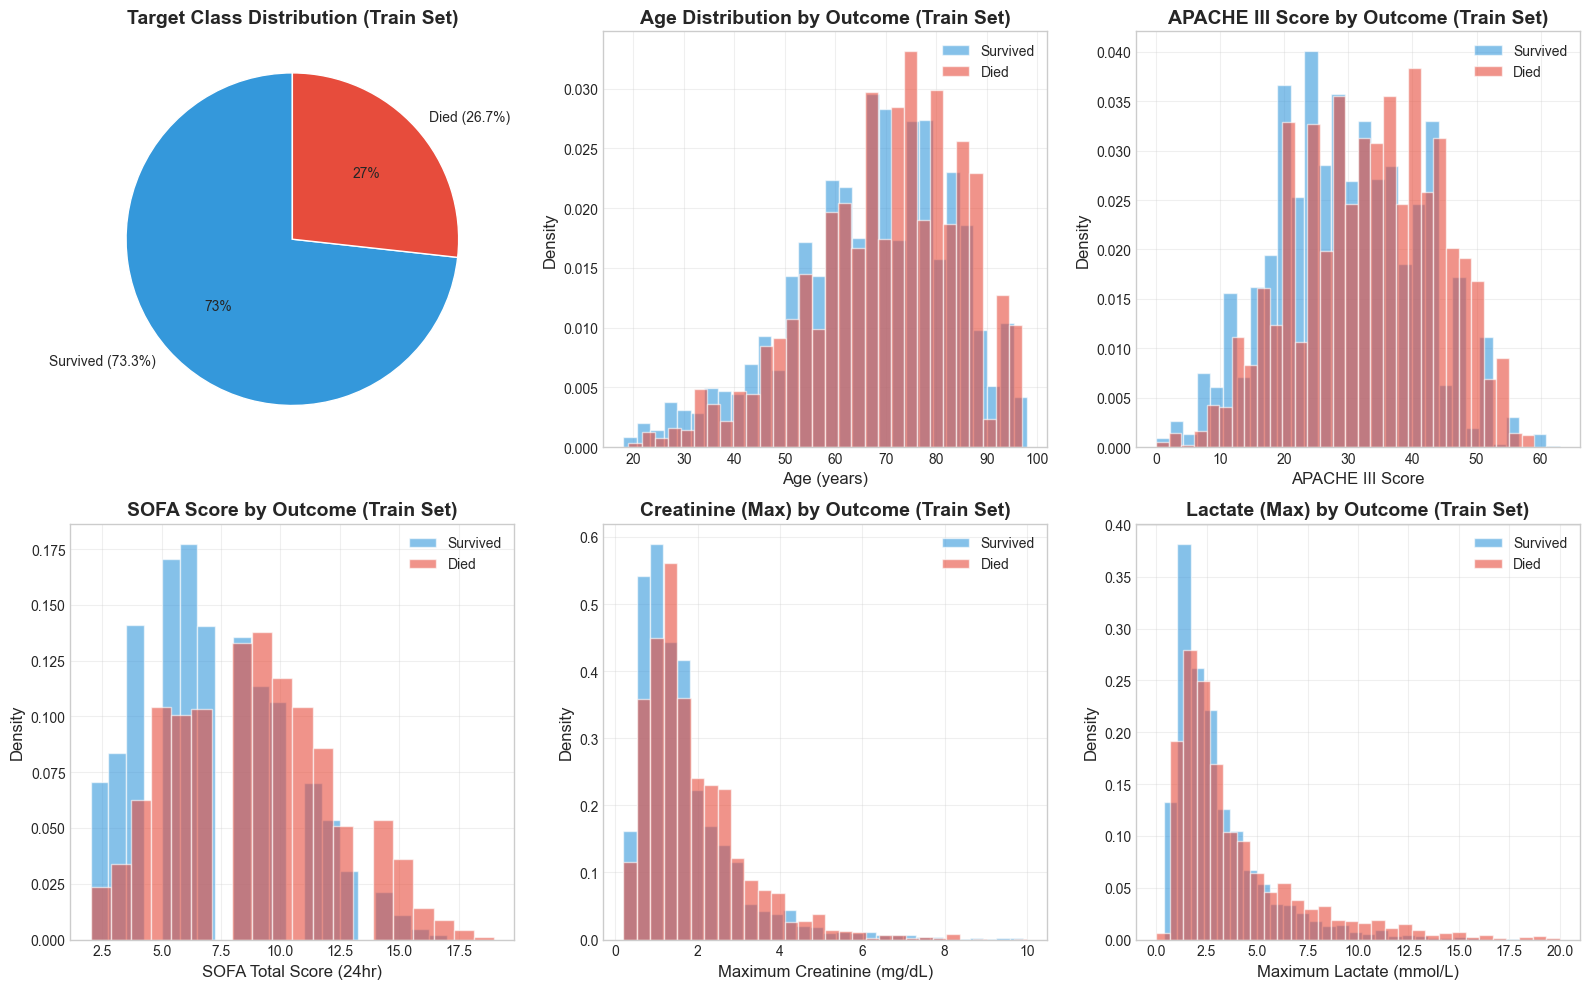
\includegraphics[width=\textwidth]{preprocessing_images/eda_distributions.png}
    \caption{Distributions of key clinical variables in the training set, stratified by mortality outcome. Non-survivors consistently show distributions shifted towards higher severity.}
    \label{fig:eda_distributions_eda}
\end{figure}

This phenotyping was further supported by correlation analysis (Figure~\ref{fig:feature_correlations_eda}). The overall SOFA score (\texttt{sofa\_total\_24hr}) had the strongest positive correlation with death (0.234), reinforcing its role as a global marker of risk. Other features strongly associated with mortality included markers of hematological dysfunction (\texttt{rdw\_median\_pct}, 0.188) and hepatic injury (\texttt{sofa\_hepatic\_24hr}, 0.169). In contrast, variables indicating physiological stability and adequate organ perfusion, such as total urine output (\texttt{urine\_output\_total\_24hr}, -0.113) and minimum pH (\texttt{ph\_min}, -0.101), were the strongest predictors of survival. Together, these findings provide a data-driven characterization of the high-risk SA--AKI patient and directly informed the feature set for supervised modeling.

\begin{figure}[htb!]
    \centering
    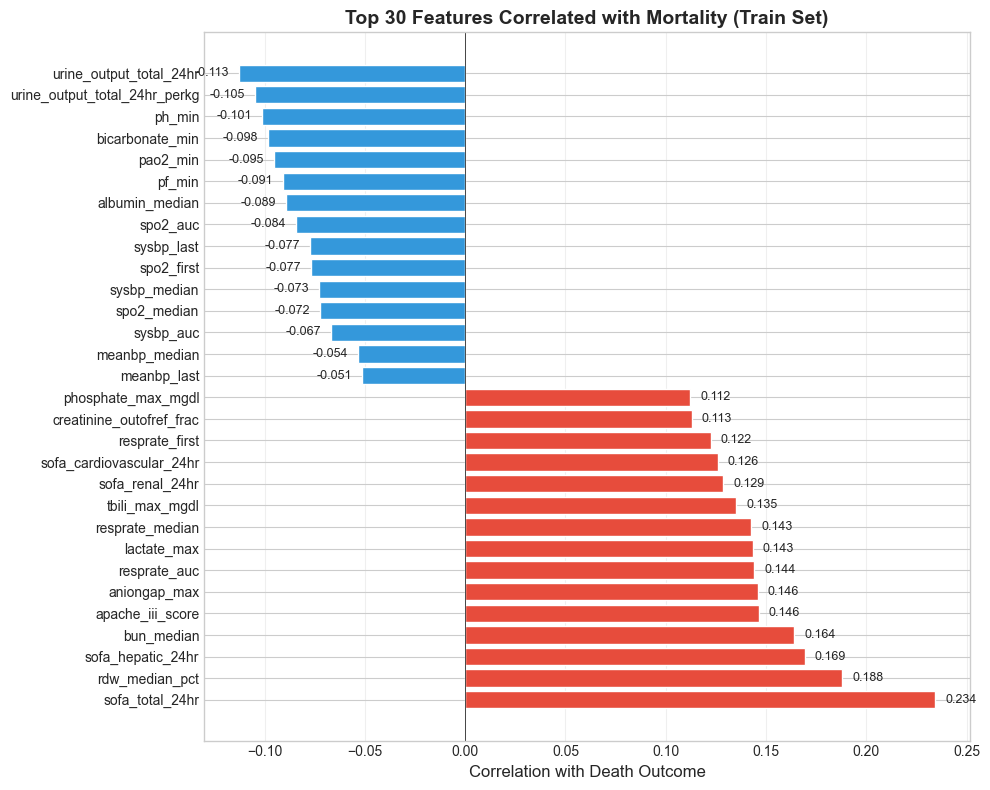
\includegraphics[width=0.8\textwidth]{preprocessing_images/feature_correlations.png}
    \caption{Top 30 features with the strongest positive (red) and negative (blue) correlation with in-hospital mortality in the training set.}
    \label{fig:feature_correlations_eda}
\end{figure}

